\appendix

\begin{frame}[allowframebreaks]
\frametitle{Références}
	\nocite{*}
	\printbibliography{}
\end{frame}

\section{Fonctionnement de l'appareil}

\begin{frame}{Cartouche pneumatique}
	\begin{columns}
	\column{0.48\textwidth}
	\begin{block}{Cartouche ouverte}
		\vspace{.25cm}
	\begin{tikzpicture}
		\pic [name=C] {cartouche};
		\pic {obturateur-bas};

		\draw [double distance=5.3mm,]
		(CO) -- ++(2,0) (CO) ++ (1,0) |- (CS)
		node [pos=0.25] {$\downarrow$}
		node [pos=0.75] {$\leftarrow$}
		;

		\draw (CI) node {$\downarrow$};
		\draw (CO) node {$\rightarrow$};

	\end{tikzpicture}
	\end{block}

	\column{0.48\textwidth}

	\begin{block}{Cartouche fermée}
		\vspace{.25cm}
	\begin{tikzpicture}

		\pic [name=C] {cartouche};
		\pic {obturateur-haut};

		\draw [double distance=5.3mm,]
		(CO) -- ++(2,0) (CO) ++ (1,0) |- (CS) 
		;

		\draw (CI) node {$\downarrow$};

	\end{tikzpicture}
	\end{block}
\end{columns}

\end{frame}

\begin{frame}[b]
	\frametitle{Circuit logique}
	\centering
	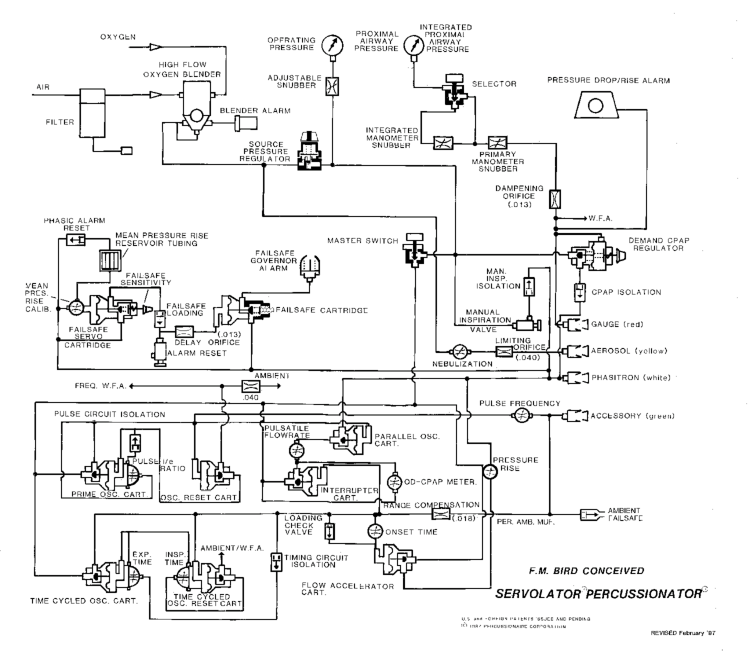
\includegraphics[height=\textheight]{img/circuit-logique.pdf}
	\note {Pas si logique que ça}
\end{frame}

\section{Analyse des tracés pression - temps}

\begin{frame}{Ratio I:E normal et inversé}
	\def\iehuit{%
\addplot graphics [
	xmin=0,
	ymin=0,
	xmax=1,
	ymax=60
]}

\begin{tikzpicture}

\begin{groupplot}[
group style={
	group size=1 by 2,
	xlabels at=edge bottom
},
enlargelimits=false,
height=0.46\textheight,
width=\textwidth,
xlabel=Temps (s),
ylabel=Pression (hPa)
]

\nextgroupplot
\iehuit {img/509.jpg};

\nextgroupplot
\iehuit{img/828.jpg};

\end{groupplot}
\end{tikzpicture}

\end{frame}

\begin{frame}{Ratio I:E normal et inversé}
	\def\iehuit{%
\addplot graphics [
	xmin=0,
	ymin=0,
	xmax=8,
	ymax=60
]}

\begin{tikzpicture}

\begin{groupplot}[
		group style={
			group size=1 by 2,
			xlabels at=edge bottom
		},
		enlargelimits=false,
		height=0.46\textheight,
		width=\textwidth,
		xlabel=Temps (s),
		ylabel=Pression (hPa)
]

\nextgroupplot
\iehuit {img/329.jpg};

\nextgroupplot
\iehuit {img/629.jpg};

\end{groupplot}
\end{tikzpicture}

\end{frame}

\begin{frame}{Augmentation des résistances}
	\centering
		\begin{tikzpicture}
		\begin{groupplot}[
				group style={
					group size=2 by 1,
					ylabels at=edge left
				},
				width=0.48\textwidth,
				restrict x to domain=1.5:4,
				every axis plot post/.style={
					mark=none
				},
				xlabel=Temps (s),
				ylabel=Pression (hPa),
				enlargelimits=false,
				ymax=40
			]
			\nextgroupplot[title=Résistances normales]
			\addplot table[x=time, y=Pao] {dat/raw5.dat};

		 \nextgroupplot[title=Résistances augmentées]
			\addplot table[x=time, y=Pao] {dat/raw15.dat};
		\end{groupplot}
	\end{tikzpicture}

\end{frame}
